\documentclass[]{book}
\usepackage{lmodern}
\usepackage{amssymb,amsmath}
\usepackage{ifxetex,ifluatex}
\usepackage{fixltx2e} % provides \textsubscript
\ifnum 0\ifxetex 1\fi\ifluatex 1\fi=0 % if pdftex
  \usepackage[T1]{fontenc}
  \usepackage[utf8]{inputenc}
\else % if luatex or xelatex
  \ifxetex
    \usepackage{mathspec}
  \else
    \usepackage{fontspec}
  \fi
  \defaultfontfeatures{Ligatures=TeX,Scale=MatchLowercase}
\fi
% use upquote if available, for straight quotes in verbatim environments
\IfFileExists{upquote.sty}{\usepackage{upquote}}{}
% use microtype if available
\IfFileExists{microtype.sty}{%
\usepackage{microtype}
\UseMicrotypeSet[protrusion]{basicmath} % disable protrusion for tt fonts
}{}
\usepackage[margin=1in]{geometry}
\usepackage{hyperref}
\hypersetup{unicode=true,
            pdftitle={Text Mining Techniques for Knowledge Extraction from Technical Documents},
            pdfauthor={Filippo Chiarello},
            pdfborder={0 0 0},
            breaklinks=true}
\urlstyle{same}  % don't use monospace font for urls
\usepackage{natbib}
\bibliographystyle{apalike}
\usepackage{longtable,booktabs}
\usepackage{graphicx,grffile}
\makeatletter
\def\maxwidth{\ifdim\Gin@nat@width>\linewidth\linewidth\else\Gin@nat@width\fi}
\def\maxheight{\ifdim\Gin@nat@height>\textheight\textheight\else\Gin@nat@height\fi}
\makeatother
% Scale images if necessary, so that they will not overflow the page
% margins by default, and it is still possible to overwrite the defaults
% using explicit options in \includegraphics[width, height, ...]{}
\setkeys{Gin}{width=\maxwidth,height=\maxheight,keepaspectratio}
\IfFileExists{parskip.sty}{%
\usepackage{parskip}
}{% else
\setlength{\parindent}{0pt}
\setlength{\parskip}{6pt plus 2pt minus 1pt}
}
\setlength{\emergencystretch}{3em}  % prevent overfull lines
\providecommand{\tightlist}{%
  \setlength{\itemsep}{0pt}\setlength{\parskip}{0pt}}
\setcounter{secnumdepth}{5}
% Redefines (sub)paragraphs to behave more like sections
\ifx\paragraph\undefined\else
\let\oldparagraph\paragraph
\renewcommand{\paragraph}[1]{\oldparagraph{#1}\mbox{}}
\fi
\ifx\subparagraph\undefined\else
\let\oldsubparagraph\subparagraph
\renewcommand{\subparagraph}[1]{\oldsubparagraph{#1}\mbox{}}
\fi

%%% Use protect on footnotes to avoid problems with footnotes in titles
\let\rmarkdownfootnote\footnote%
\def\footnote{\protect\rmarkdownfootnote}

%%% Change title format to be more compact
\usepackage{titling}

% Create subtitle command for use in maketitle
\newcommand{\subtitle}[1]{
  \posttitle{
    \begin{center}\large#1\end{center}
    }
}

\setlength{\droptitle}{-2em}

  \title{Text Mining Techniques for Knowledge Extraction from Technical Documents}
    \pretitle{\vspace{\droptitle}\centering\huge}
  \posttitle{\par}
    \author{Filippo Chiarello}
    \preauthor{\centering\large\emph}
  \postauthor{\par}
      \predate{\centering\large\emph}
  \postdate{\par}
    \date{2018-09-11}

\usepackage{booktabs}

\begin{document}
\maketitle

{
\setcounter{tocdepth}{1}
\tableofcontents
}
\chapter{Introduction}\label{introduction}

\section{Goal}\label{goal}

Il problema non è sostituire domain knowledge. Idea vecchia ha fallito.
E' insostibuibile perchè:

\begin{itemize}
\tightlist
\item
  Technology, interessa gli ingegneri
\item
  Social Science, decision making
\end{itemize}

PErchè fallita: da una parte è andata avanti la knowledge
rappresentation. E' impossibile rappresentare la conoscenza con regole,
ma con altri strumenti si può rappresentare (bottom-up).

Inoltre ho text mining, capaità di processare testi. Parte di
intelligenza artificiale. Questi fenomeni non sostituioscono l'esperto
ma ne cambiano il modo di operare.

Oggi si integra. Vogliamo un esperto di dominio che faccia meglio il suo
mestiere.

Abbiamo oggi più potenza e correzione errori.

Oltre ad efficienza e potenza nel correggere gli errori. Ora c'è anche
la possibilità dio maggiore specificità. L'obiettivo è qiuindi poratre
domain knowledge sia su technology sia ai decisori sociali.

\section{Problem}\label{problem}

Foresight

\section{Solutions}\label{solutions}

\begin{figure}

{\centering 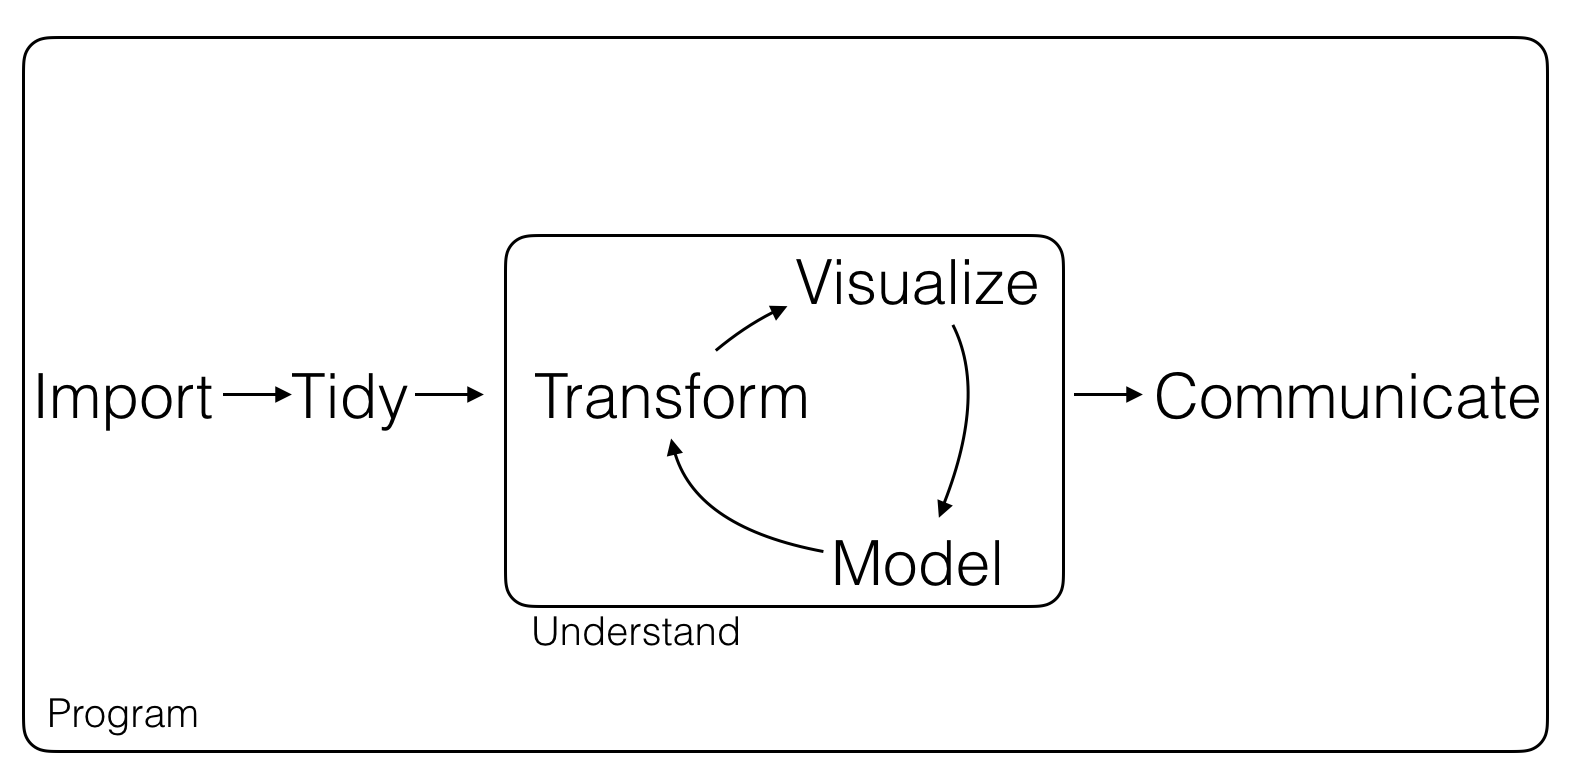
\includegraphics[width=0.8\linewidth]{_bookdown_files/figures/main_work_flow} 

}

\caption{A general workflow for the process of data analysis. Readapted from Wickham (2016)}\label{fig:mainworkflow}
\end{figure}

\section{Challenges: Understanding and
Programming}\label{challenges-understanding-and-programming}

\subsection{Understanding}\label{understanding}

\subsection{Programming}\label{programming}

\section{Research Questions}\label{research-questions}

\section{Stakeholders}\label{stakeholders}

Marketing

Research and Development

Design

Human Resources

Other Stakeholders

\section{Knowledge Intensive Manegement
Engineering}\label{knowledge-intensive-manegement-engineering}

Tipicamente occupaimo di attività ad altà ripetitività. Ti porti dietro
metodologie ingegneristiche applicate a sistemi inernti, andnano a
operare in sistemi socio-tecnici. Hai fatto il tuo mestieri (ricerca
operativa ecc..). Negli ultimi anni però le aziende le attività a
maggior valore aggiunto sono non ripetitive. R\&S, Design, marketing, HR
ecc.. e quindi gestione della conoscena. Su situazione che sembrano
uniche il gestionale rischia di perdere rispetto al creativo. Come
disciplina voglio presidiare queste aree: non ci occupaimo di casi
unici, ma costruire modelli in grado di incorporare conoscenza per
essere usati in questi. La tesi ha l'obbiettivo di esploration and
exploitation queste direzioni. Hon trovato nella data science è più
nello specifico nel text mining gli strumenti adatti.

\chapter{State of the Art}\label{sota}

The analysis of technical documents require the design of processes that
rely both on programming and Natural Language Processing techniques and
on the undestanding and knowldege of field experts. While the first
techniques are codified and explicit, the second are sometimes implicit
and always harder to systematize. In this section i treat these two
groups of techniques in the same way to give to the reader a sistematic
litterature review on these topics. For this reason the sections of this
chapter has the sequent structure:

\begin{itemize}
\tightlist
\item
  At a first level we have two sections \ref{sotatools} and
  \ref{sotadocuments}, reviewing respectivelly the processes of
  \emph{programming and Natural Language Processing} and of
  \emph{undestanding and knowldege of field experts application};
\item
  Section \ref{sotatools} has a subsection for each of the \emph{phases}
  showed in figure \ref{fig:mainworkflow}. These subsections goes from
  \ref{sotatoolsprogram} to \ref{sotatoolscomunicate};
\item
  Each subsection from \ref{sotatoolsprogram} to
  \ref{sotatoolscomunicate} contains the relative Natural Language
  Processing \emph{task} that are relevant for the analysis of technical
  documents, for example Document Retrieval
  \ref{sotatoolsimportretrieval}, Part-Of-Speech-Tagging;
  \ref{sotatoolstransformpos} or Named Entity Recognition
  \ref{sotatoolsmodelner}.
\item
  Each task subsection describes the relevant \emph{techniques} to
  perform that task. I use the word techniques to include mainly
  algorythms and procedures but also more generic methods or frameworks;
\item
  Since the second section \ref{sotadocuments} describes less
  systematics phases, task and techniques this section opens with a
  first subsection \ref{sotadocumentsunderstand} that focuses on the
  studies of the problems of using expert knowledge in an analytical
  process and which are the techniques to convert this knowledge in a
  format that is usable in a Natural Language Processing workflow.
\item
  Finally, always section \ref{sotadocuments} has a subsection for each
  of the technical \emph{documents} I analyzed (aggiungi gancio con
  introduzione). These subsections goes from \ref{sotadocumentspatents}
  to \ref{sotadocumentsjobs}.
\end{itemize}

\section{Phases, Tasks, and Techniques}\label{sotatools}

In this section I make a review of the most important techniques for
Natural Language Processing in the context of technical documents
analysis. The techniques (mainly algorythms) are grouped in phases
(Import, Tidy, Transform, Model, Visualize, Communicate) showed in
figure \ref{fig:mainworkflow} and each phases is dived in the NLP tasks
that are the most important for the analysis of technical documents. The
algorythms i reviewed in this section are summmarised in table tot,
where the reader can see the relationship between tasks and techniques.

\subsection{Program}\label{sotatoolsprogram}

\begin{itemize}
\tightlist
\item
  \textbf{Articoli Emily}
\end{itemize}

\subsection{Import}\label{sotatoolsimport}

\begin{itemize}
\tightlist
\item
  I tipi di codifica di testo
\item
  Pachetti per import
\end{itemize}

\subsubsection{Document Retrieval}\label{sotatoolsimportretrieval}

\begin{itemize}
\tightlist
\item
  Letteratura query
\end{itemize}

\subsection{Tidy}\label{sotatoolstidy}

\begin{itemize}
\tightlist
\item
  Hadley
\end{itemize}

weight, tfids

DTM

problems such as sparsity

\subsection{Transform}\label{sotatoolstransform}

Transforming in the context of Natural Language Processing is what in
computational linguistic is called text normalization. Normalizing text
means converting it to a more convenient, standard form. Most of the
task of technical document analysis in fact relies on first separating
out or tokenizing sentences and words, strip suffixes from the end of
the word, determining the root of a word or transform the text using
regular expressions.

\subsection{Sentence Splitting}\label{sentence-splitting}

The analysis of technical documents require as first process, that the
input text is segmented in sentences. Since documents do not encode this
information in a non ambiguous manner (using dots) due to common
abbreviations (e.g.: ``Mr., Dr.''), a sentence splitting process that
does not rely only on a trivial \emph{dot based} rule is required. This
issue in the technical documents domain is even more problematic due to
the presence of formulas, numbers, chemical entity names and
bibliographic references. Furthermore, since sentece splitting is one of
the first processes of an NLP pipeline, errors in this early stage are
propagated in the following steps causing a strong decrease for what
concerns their accuracy. One of the most advanced techniques are machine
learning techniques: given a training corpus of properly segmented
sentences and a learning algorithm, a statistical model is built. By
reusing the statistical model, the sentence splitter is able to split
sentences on texts not used in the training phase. ItalianNLP lab
systems uses this approach
\citep{dell2009ensemble, attardi2009reverse, attardi2009accurate}. For
this reason this algorythm is used for the most of the application
presented in this Thesis.

\subsection{Tokenization}\label{tokenization}

Since documents are unstructured information, these has to be divided
into linguistic units. The definition of linguistic units is
non-trivial, and more advanced techniques can be used (such as n-gram
extraction) but most of the times these are words, punctuation and
numbers. English words are often separated from each other by
whitespace, but whitespace is not always sufficient. Solving this
problems and splitting words in well-defined tokensis defined as
tokenization. In most of the application described in the present
Thesis, the tokenizer developed by the ItalianNLP lab was integrated
\citep{dell2009ensemble, attardi2009reverse, attardi2009accurate}. This
tokenizer is regular expression based: each token must match one of the
regular expression defined in a configuration file. Among the others,
rules are defined to tokenize words, acronyms, numbers, dates and
equations.

\subsubsection{Stemming}\label{sotatoolstransformstemming}

Stemming is a simpler but cruder methodology for chopping off of
affixes. The goal of stemming is reducing inflected (or sometimes
derived) words to their word stem, base or root form. The stem of a word
and its morphological root do not need to be identical; it is sufficient
that related words map to the same stem, even if this stem is not a
valid root. One of the most widely used stemming is the simple and
efficient Porter algorithm \citep{porter1980algorithm}.

\subsubsection{Lemmatisation}\label{sotatoolstransformlemmatisation}

Lemmatization is the task of determining the root of a words. The output
allow to find that two words have the same root, despite their surface
differences. For example, the verbs \emph{am}, \emph{are}, and \emph{is}
have the shared lemma \emph{be}; the nouns \emph{cat} and \emph{cats}
both have the lemma \emph{cat}. Representing a word by its lemma is
important for many natural language processing tasks. Lemmatisation in
fact diminish the problem of sparsity of document-word matrix.
Futhermore lemmatisaion is important for document retrieval
\ref{sotatoolsimportretrieval} web search, since we want to find
documents mentioning motors if we search for motor. The most recent
methods for lemmatization involve complete morphological parsing of the
word \citep{hankamer1989morphological}.

\subsubsection{Part-of-Speech Tagging}\label{sotatoolstransformpos}

The part of speech plays an central role in technical document analysis
since it provides very useful information concerning the morphological
role of a word and its morphosyntactic context: for example, if a token
is a determiner, the next token is a noun or an adjective with very high
confidence. Part of speech tags are used for many information extraction
tools such as named entity taggers (see section \ref{sotatoolsmodelner})
in order to identify named entities. In typical named entity task these
are people and locations since tokens representing named entities follow
common morphological patterns (e.g.~they start with a capital letter).
For the application to technical documents, technical entities (like the
possibile failures of a manufact) becomes more relevant. In this context
a correct part-of-speech tagger becomes even more important since we can
not rely on morphosyntactical rules. In addition part of speech tags can
be used to mitigate problems related to polysemy since words often have
different meaning with respect to their part of speech (e.g. ``track'',
``guide''). This information is extremelly valuable in patent analysis,
and some patent tailored part-of-speech tagger has been designed (see
section \ref{sotadocumentspatents}). The litterature on pos-tagger is
huge, and goes behoind the scope of the present thesis to make a
complete review. In most of the application presentend in this work, was
employed the ILC postagger \citep{attardi2006experiments}. This
postagger uses a supervised training algorithm: given a set of features
and a training corpus, the classifier creates a statistical model using
the feature statistics extracted from the training corpus.

\subsubsection{Regular Expressions}\label{sotatoolstransformregex}

Regular expression (regex) is a language for specifying text search
strings, an algebraic notation for characterizing a set of strings. This
language whidelly used in modern word processor and text processing
tools.. They are particularly useful for searching in texts, when we
have a pattern to search for.

A pattern could be at A regular expression search function will search
through the corpus, returning all texts that match the pattern. The
corpus can be a single document or a collection. For example, the Unix
command-line tool grep takes a regular expression and returns every line
of the input document that matches the expression. A search can be
designed to return every match on a line, if there are more than one, or
just the first match. In the following examples we generally underline
the exact part of the pattern that matches the regular expression and
show only the first match. We'll show regular expressions delimited by
slashes but note that slashes are not part of the regular expressions.

\subsection{Model}\label{sotatoolsmodel}

Classi di modelli. Pedro Domingos

\citep{james2013introduction}

\subsubsection{N-Grams}\label{sotatoolstransformngrams}

An n-gram is a sequence of N n-gram words: a 2-gram (or bigram) is a
two-word sequence of words like ``credit card'', ``3d printing'', or
''printing machine'', and a 3-gram (or trigram) is a three-word sequence
of words like ``3d printing machine''. Statistical model can be used to
extract the n-grams contained in a document. A first approach has the of
predicting the next item in a sequence in the form of a (n − 1)--order
Markov model\citep{lafferty2001document}. The algorythm begin with the
task of computing P(w\textbar{}h), the probability of a word w given a
word h.The way to extimate this probability is using relative frequency
counts. To do that the algorythms count the number of times h is
followed by the w. With a large enough corpus it is possibile to build
valuable models, able to extract n-grams
\citep{bellegarda2004statistical}. While this method of estimating
probabilities directly from counts works for many natural language
applications, in many cases a huge dimension of the corpus does make the
model useful, and this is particularly true for technical documents
\citep{brants2012large}. This is because technical language has a strong
ratio of evolution; as new artifcat are invented, new chunks are created
all the time, and has no sense to continuolly count every word
co-occurrence to update our model\citep{gibson1994tools}. A more usefull
method for chunk extraction fro technical document uses
part-of-speech-tagging and regular expression. Once a document is
pos-taggerd each word is associated whit a particular part of speech:
each sentence is rapresented as a sequence of part-of-spech. Once we
have this rappresentation, it is possible to etract only certain
sequences of part-of-speeches, the ones that whit an high level of
confidence are n-grams.

{[}TROVA LAVORI SU QUESTO ARGOMENTO{]}

\subsubsection{Document Classification}\label{sotatoolsmodeldocclass}

Classification is a general process that has the goal of taking an
object, extract features, and assign to the observation one of a set of
discrete classes. This process is largerly used for documents
\citep{borko1963automatic} and there exist many methods for document
classification \citep{aggarwal2012survey}.

Regardless of technological sector, most organizations today are facing
the problem of overload of information. When it comes to classify huge
ammount of documents or to separate the useful documents from the
irrelevant, document classification techniques can reduce the proecess
cost and time.

The simplest method for classifying text is to use expert defined rules.
These systems are called expert systems or knowledge engineering
approach. Expert rule-based systems are programs that consist of rules
in the IF form condition THEN action (if condition, then action). Given
a series of facts, expert systems, thanks to the rules they are made of,
manage to deduce new facts. The expert systems therefore differ from
other similar programs, since, by referring to technologies developed
according to artificial intelligence, they are always able to exhibit
the logical steps that underlie their decisions: a purpose that, for
example, is not feasible from the human mind or black box-systems. There
are many type of documents for which expert based classifiers constitute
a stateof-the-art system, or at least part of it. Anyway, rules can be
useless in situations such as: - data change over time - the rules are
too many and interrelated

Most systems of documents classification are instead done via supervised
learning: we have a data set of input observations, each associated with
some correct output (training set). The goal of the algorithm is to
build a statical model able to learn how to map from a new observation
(test set) to a correct output. The advantages of this approach over the
knowledge engineering approach are a very good effectiveness,
considerable savings in terms of expert labor power, and straightforward
portability to different domains.

In the supervised document classification process, we have a training
set of N documents that have each been tipically hand-labeled with a
class: (d1, c1),\ldots{}.,(dN, cN). I say tipically, because other less
expensive methods could be designed, as we will show for the task of
Named Entity Recongition (another supervised learning task, that
classifies words intstead of documents \ref{sotatoolsmodelner}). The
goal of the supervised document classification task is to learn a
statistical model capable of assign a new document d to its correct
class c ∈ C. There exist a class of these classifier, probabilistic
classifiers, that additionally will tell us the probability of the
observation being in the class.

Many kinds of machine learning algorithms are used to build classifiers
\citep{aggarwal2012survey}, such as:

\begin{itemize}
\item
  \emph{Decision Tree Classifiers}: Decision tree documents classifier
  are systems that has as output a classification tree
  \citep{sebastiani2002machine}. In this tree internal nodes are terms
  contained in the corpus under analysis, branches departing are labeled
  by the weight (see section \ref{sotatoolstidy}) that the term has in
  the test document, and leafs are labeled by categories. There exists
  many methods to automatically learn trees from data. A tree can be
  build by splitting the data source into subsets based on an test
  feature. This process is repeated on each derived subset in a
  recursive manner called recursive partitioning. The recursion is
  completed when the subset at a node has all the same value of the
  target variable, or when splitting no longer adds value to the
  predictions.
\item
  \emph{Rule Based Classifiers}: Rule-based classifiers are systems in
  wich the patterns which are most likely to be related to the different
  classes are extracted from a set of test documents. The set of rules
  corresponds to the lefthand side to a word pattern, and the right-hand
  side to a class label. These rules are used for the purposes of
  classification. In its most general form, the left hand side of the
  rule is a boolean condition, which is expressed in Disjunctive Normal
  Form (DNF). However, in most cases, the condition on the left hand
  side is much simpler and represents a set of terms, all of which must
  be present in the document for the condition to be satisfied
  \citep{yang2004building}.
\item
  \emph{Support Vector Machines (SVM) Classifiers}: SVM Classifiers
  attempt to partition the data space with the use of linear or
  non-linear delineations between the different classes. The main
  principle of SVM algorythm is to determine separators in the feature
  space which can best separate the different classes
  \citep[\citet{manevitz2001one}]{joachims1998text}.
\item
  \emph{Baeysian Classifiers}: Bayesian classifiers build a
  probabilistic classifier based on modeling the underlying word
  features in different classes. The idea is then to classify documents
  using the posterior probability of the documents belonging to the
  different classes on the basis of the word presence in the documents
  \citep{pop2006approach}.
\item
  \emph{Neural Netword Classifiers}: The basic unit in a neural network
  is a neuron. Each neuron receives a set of inputs, which are denoted
  by the vector \emph{Xi}, which are the values of the feature vector
  for a certain instance. Each neuron is also associated with a set of
  weights, which are used in order to compute a function of its inputs.
  Neural Networks Classifier are able, thank to a process called
  learning phase, to ajust their weights in such a way that the function
  is abble to effectively classify new instances. Neural networks are
  nowdays one of the best method for documents classification, and are
  used in a wide variety of appliations \citep{manevitz2007one}. Great
  performances has also been reached by deep neural networks, which are
  neural networks whit a large number o neurons arranged in multiple
  layers \citep[\citet{kim2014convolutional}]{lai2015recurrent}.
\end{itemize}

\subsubsection{Sentiment Analsysis}\label{sotatoolsmodelsentanal}

Sentiment analysis techniques are algorythms able to measure from text,
people's opinions and emotions toward events, topics, products and their
attributes \citep{pang2008opinion}. For example, businesses
(particularly marketeers) are intrested in finding costumers opinions
about their products and services.

Thanks to the growth of social media (forums, blogs and social
networks), individuals and organizations are producing a huge quantity
of their written opinion. This has make it possible to scholars to study
this phenomena and to develop many different and effective sentiment
analysis techniques \citep{liu2012survey}. In the past decade, a
considerable amount of research has been done by scholars and there are
also numerous commercial companies that provide opinion mining services.
However, measuring sentiment in documents and distilling the information
contained in them remains a challenging task because of the diversity of
documents from which is possibile to extract sentiment.

The approaches to perform sentiment analysis are many. Among all, the
most intresting for tehcnical documents analysis are:

\begin{itemize}
\item
  \emph{Dictionary Base Approaches} : This approach has the aim of
  collecting words that are clues for positive or negative sentiment. In
  litterature these words are called opinion words, opinion-bearing
  words or sentiment words. Examples of positive opinion words are:
  good, nice and amazing. Examples of negative opinion words are bad,
  poor, and terrible. Collectively, they are called the opinion lexicon.
  The most simple and widely used techniques to produce a dictionary of
  opinion words is based on bootstrapping using a small set of seed
  opinion words and an online dictionary such as WordNet
  \citep{miller1995wordnet}. The works that used this approach
  \citep[\citet{kim2004determining}]{hu2004mining}, adopts a process
  that consist in two phases: first collect set of opinion words
  manually, then grow this set by searching in the WordNet for their
  synonyms and antonyms. The process stops when no more new words are
  found. After that a manual inspection can be carried out to remove
  and/or correct errors. Scholars has developed several opinion lexicons
  \citep[\citet{baccianella2010sentiwordnet}, \citet{hu2004mining},
  \citet{philip1966general},
  \citet{wiebe1999development}]{ding2008holistic} The lexicon based
  approach has the characteristic of beeing strongly context specific.
  This is an advantage when the goal is to design a method able to
  extract sentiment in a specific context \citep{chiarello2017product},
  but is a major shortcoming if the goal is to design a general purpose
  method.
\item
  \emph{Supervised Learning Approaches}:
\item
  \emph{Corpus-based Approaches}
\end{itemize}

\subsubsection{Network Analysis}\label{sotatoolsmodelnetanal}

\subsubsection{Named Entity Recognition}\label{sotatoolsmodelner}

\subsubsection{Topic Modelling}\label{sotatoolsmodeltopicmodel}

\subsection{Visualize}\label{sotatoolsvisualize}

\subsection{Comunicate}\label{sotatoolscomunicate}

\section{Documents}\label{sotadocuments}

\subsection{Understand}\label{sotadocumentsunderstand}

Expertise (collins)

Sheela Jasanow

Taleb?

\subsubsection{The problem of byases}\label{sotadocumentsunderstandbyas}

Each site typically contains a huge volume of opinionated text that is
not always easily deciphered in long forum postings and blogs. The
average human reader will have difficulty identifying relevant sites and
accurately summarizing the information and opinions contained in them.
Moreover, it is also known that human analysis of text information is
subject to con- siderable biases, e.g., people often pay greater
attention to opinions that are consistent with their own preferences.
People also have difficulty, owing to their mental and physical
limitations, producing consistent results when the amount of information
to be processed is large. Automated opinion mining and summarization
systems are thus needed, as subjective biases and mental limitations can
be overcome with an objective sentiment analysis system.

\subsubsection{The Importance of Lexicons for Technical Documents
Analysis}\label{sotadocumentsunderstandlexicons}

\subsubsection{Expert Systems}\label{expert-systems}

\subsection{Patents}\label{sotadocumentspatents}

\subsection{Papers}\label{sotadocumentspapers}

\begin{itemize}
\tightlist
\item
  Parte Barilari.Keyword base, defini i confini di area tecnologica.
  Hot-topics su paper (guaiè)
\item
  Biblio
\end{itemize}

\subsection{Projects}\label{sotadocumentsprojects}

\subsection{Wikipedia}\label{sotadocumentswiki}

\subsection{Twitter}\label{sotadocumentstwitter}

\subsection{Job Profiles}\label{sotadocumentsjobs}

\chapter{Methods}\label{methods}

In this chapter I describe the methods applied for the analysis of
different types of documents containing technical information. The
methods are ensamble of Natural Language Processing (NLP) and Text
Mining techniques described in @ref(sota\_tools), re-designed depending
on the analyzed document and the analysis goal.

Table tot summarise the relations between the documents under analysis
(introduced in section @ref(sota\_documents)) and the NLP techniques.

Table documents vs tools

Table algorithms vs tools

\section{Patents}\label{patents}

\section{Papers}\label{papers}

\section{Projects}\label{projects}

\section{Wikipedia}\label{wikipedia}

\section{Twitter}\label{twitter}

\section{Job Profiles}\label{job-profiles}

\chapter{Applications and Results}\label{applications-and-results}

Some \emph{significant} applications are demonstrated in this chapter.

\section{Patents}\label{patents-1}

\section{Papers}\label{papers-1}

\section{Projects}\label{projects-1}

\section{Wikipedia}\label{wikipedia-1}

\section{Twitter}\label{twitter-1}

\section{Job Profiles}\label{job-profiles-1}

\chapter{Future Developments}\label{future-developments}

\section{Marketing}\label{marketing}

\section{Research and Development}\label{research-and-development}

\section{Design}\label{design}

\section{Human Resources}\label{human-resources}

\chapter{Conclusions}\label{conclusions}

We have finished a nice thesis

\chapter{Glossary}\label{glossary}

Morphology= the study of the way words are built up from smaller
meaning-bearing units called morphemes.

\bibliography{papers.bib}


\end{document}
